% !TEX root = main.tex
\documentclass[12pt]{article}

% Preamble (packages + macros)
\usepackage[utf8]{inputenc}
\usepackage{amsmath, amssymb, amsthm}
\usepackage{tikz}
\usepackage{enumitem}
\usepackage[
    colorlinks=true,
    linkcolor=blue,
    citecolor=blue,
    urlcolor=blue
]{hyperref}
\usepackage[none]{hyphenat}
\usepackage{multicol}

% Larger margin on the right for handwritten notes
\usepackage[
    left=1.0in,
    right=1.5in,
    top=1in,
    bottom=1in
]{geometry}

% Slightly nicer spacing but still classic
\linespread{1.15}

% Section spacing minimal
\usepackage{titlesec}
\titlespacing*{\section}{0pt}{1.5ex}{0.8ex}
\titlespacing*{\subsection}{0pt}{1ex}{0.5ex}

% No colored boxes, no fancy fonts

% ==========================================
% 1. Custom Layout Environments (No numbering)
% ==========================================

\newenvironment{goal}
  {\noindent\textbf{Goal.}}
  {\par\vspace{0.75em}}

\newenvironment{subgoal}
  {\noindent\textbf{Subgoal.}}
  {\par\vspace{0.75em}}

\newenvironment{idea}
  {\noindent\textbf{Idea.}}
  {\par\vspace{0.75em}}

\newenvironment{solution}
  {\noindent\textbf{Solution.}}
  {\par\vspace{0.75em}}

% ==========================================
% 2. Standard Theorem Environments (amsthm)
% ==========================================

% --- Style A: PLAIN (Bold title, Italic body) ---
% Best for: Theorems, Lemmas, Corollaries, Propositions
\theoremstyle{plain}
\newtheorem{theorem}{Theorem}[section]      % Resets counter per section (e.g., 1.1)
\newtheorem{lemma}[theorem]{Lemma}          % Shares counter with Theorem
\newtheorem{corollary}[theorem]{Corollary}
\newtheorem{proposition}[theorem]{Proposition}

% --- Style B: DEFINITION (Bold title, Upright body) ---
% Best for: Definitions, Examples, Remarks
\theoremstyle{definition}
\newtheorem{definition}{Definition}[section]
\newtheorem{example}{Example}[section]
\newtheorem{remark}{Remark}[section]

% ==========================================
% 3. Legacy/Custom Compatibility
% ==========================================

% This preserves your old 'mydef' style (Bold title, Newline, Upright body)
% You can use this if you prefer the newline after the title, 
% or migrate to the standard \begin{definition} above.

\newtheoremstyle{mydefstyle}
  {1em}{1em}   % Space above/below
  {}           % Body font (empty = upright)
  {}           % Indent amount
  {\bfseries}  % Theorem head font
  {}           % Punctuation after head
  {\newline}   % Space after head (newline)
  {}           % Head spec

\theoremstyle{mydefstyle}
\newtheorem{mydefinition}{Def.}[section]

% Wrapper environment to match your previous files
\makeatletter
\newenvironment{mydef}[1][]
  {\begin{mydefinition}[#1]}
  {\end{mydefinition}}
\makeatother
\setcounter{tocdepth}{1}

\begin{document}
\author{}

% Title
\title{
    \vspace{2cm} 
    {\Large DS-GA 1014}\\[0.5em]
    {\Large Optimization and Computational Linear Algebra}\\[0.5em]
    {\large Andrew Liao}\\[0.5em]
    {\large \today}\\[0.5em]
}
\date{} 
\maketitle
\newpage

% ---- Abstract ----
\section*{Abstract}
\addcontentsline{toc}{section}{Abstract}

This is a graduate level, proof-based linear algebra course taught by \href{https://florentinguth.github.io/}{Florentin Guth} at NYU Center for Data Science. 
It covers the basics of optimization and computational linear algebra in Data Science applications, with 66\% of content being linear algebra and 33\% being optimization.
This course was taken in Fall of 2025, with the date in title page indicating date last updated. 
\vspace{5cm}

\begin{center}
    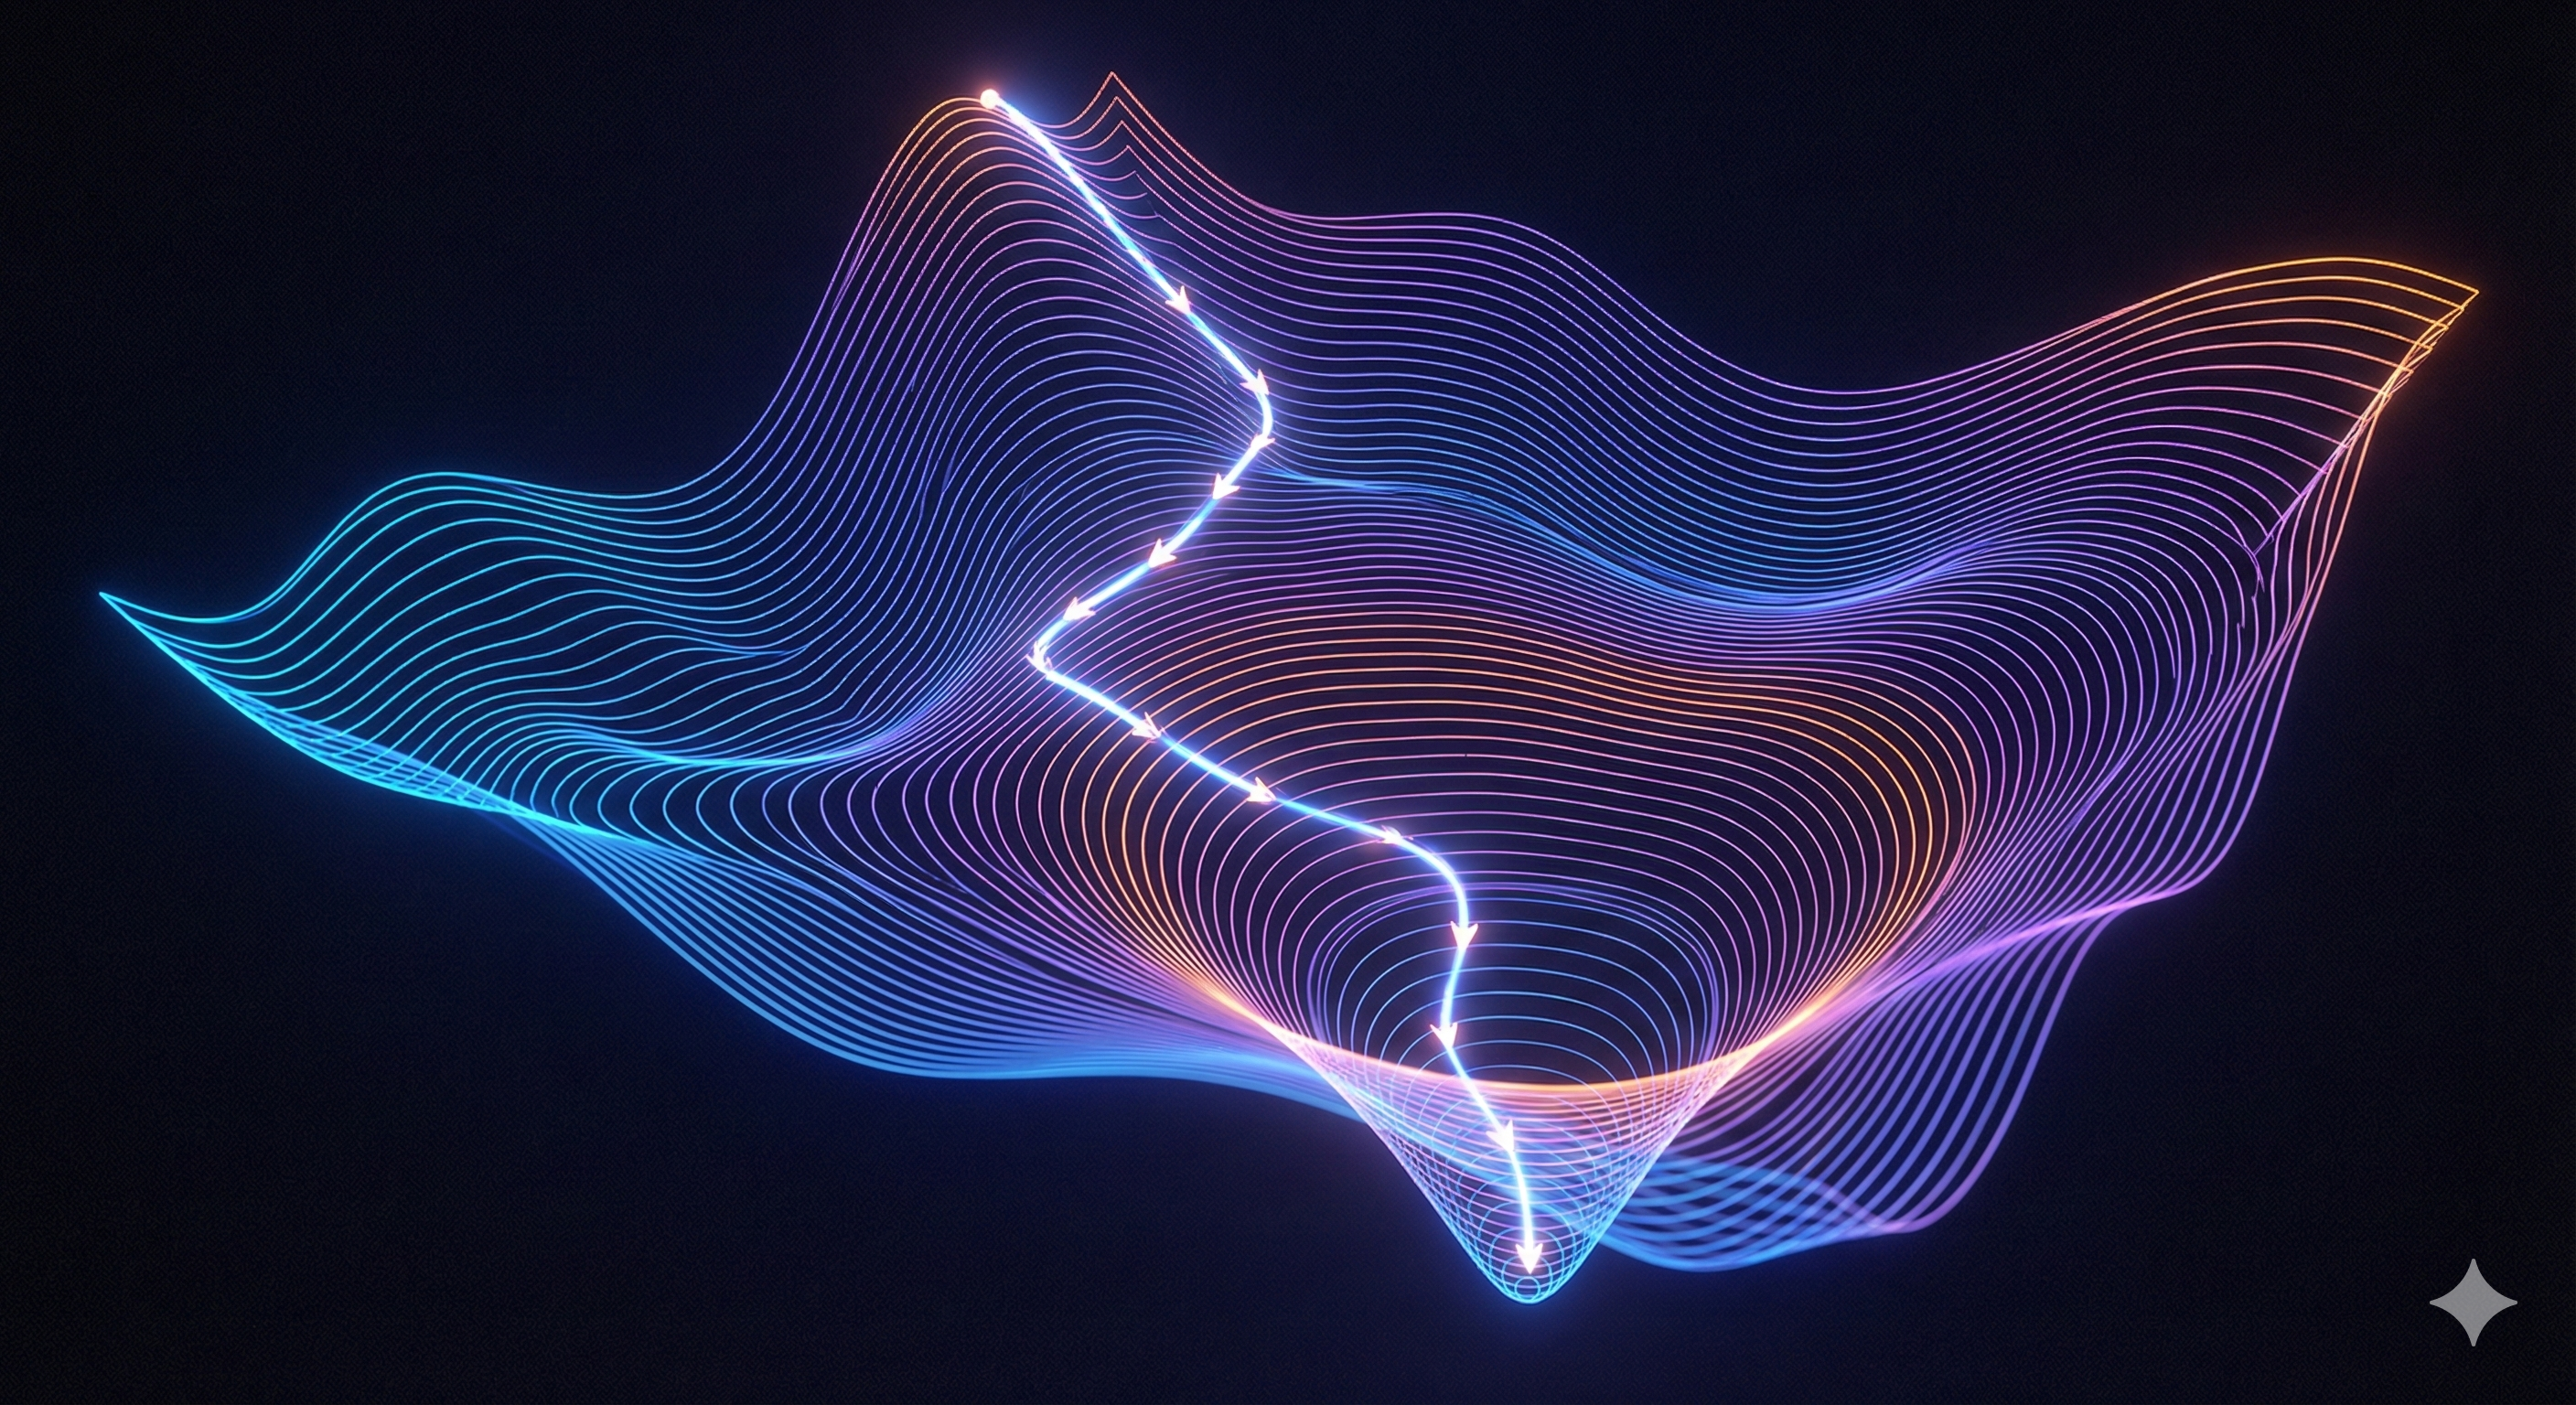
\includegraphics[width=\textwidth]{LA_opt_cover.png}
\end{center}

\vspace{10em}
\noindent Image generated with Nano Banana Pro with prompt: "cool gradient descent figure".
\newpage

% Table of contents
\tableofcontents
\newpage

% ---- Lectures ----
% !TEX root = ../main.tex
\section{Vector Spaces}

\subsection{Vector Spaces}

\begin{definition}[Vector]
    A \textbf{vector} $\bar{v}$ is a mathematical object defined by the operations of vector addition and scalar multiplication. Vectors have a geometric interpretation as arrows in space and a numerical interpretation as ordered lists of real numbers.
\end{definition}

\begin{definition}[Vector Space]
    A \textbf{vector space} $V$ is a set of vectors satisfying the following axioms for all $x,y,z \in V$ and scalars $a,b,c,d \in \mathbb{R}$:
    \begin{multicols}{2}
    \begin{enumerate}
        \item Closure under addition: $x+y \in V$
        \item Commutativity: $x+y = y+x$
        \item Associativity: $(x+y)+z = x+(y+z)$
        \item Additive identity: $\exists\,0 \in V$ such that $x+0=x$
        \item Additive inverse: $\exists\,(-x)\in V$ such that $x+(-x)=0$
        \item Closure under scalar multiplication: $cx \in V$
        \item Compatibility: $c(dx) = (cd)x$
        \item Multiplicative identity: $1 \cdot x = x$
        \item Distributivity: $a(x+y)=ax+ay$
        \item Scalar distributivity: $(a+b)x=ax+bx$
    \end{enumerate}
    \end{multicols}
    Both vectors and vector spaces are defined through operations rather than representation.
\end{definition}

\begin{definition}[Subspace]
    A \textbf{subspace} $S\subseteq V$ is a subset that:
    \begin{enumerate}
        \item contains the zero vector,
        \item is closed under vector addition,
        \item is closed under scalar multiplication.
    \end{enumerate}
    If these conditions hold, $S$ is a vector space.
\end{definition}

\subsubsection*{Examples}
\begin{itemize}
    \item $\mathbb{R}^n$ is a subspace of itself.
    \item $\{0\}$ is a subspace of any vector space.
    \item Any line through the origin is a subspace of $\mathbb{R}^2$.
\end{itemize}

\subsection{Span and Linear Dependence}

\begin{definition}[Linear Combination]
    A vector $y\in V$ is a \textbf{linear combination} of $x_1,\dots,x_k$ if
    \[
    y=\sum_{i=1}^{k}\alpha_i x_i,
    \]
    for scalars $\alpha_i\in\mathbb{R}$.
\end{definition}

\begin{definition}[Span]
    The \textbf{span} of vectors $x_1,\dots,x_n$ is the set of all linear combinations.
    \[
    \operatorname{span}(x_1,\dots,x_n)
    = \{ \alpha_1x_1 + \dots + \alpha_nx_n : \alpha_i\in\mathbb{R}\},
    \]
    the smallest subspace of $V$ that contains them.
\end{definition}

\begin{definition}[Linear Dependence]
    Vectors $x_1,\dots,x_k$ are \textbf{linearly dependent} if not all scalars
    $\alpha_1,\dots,\alpha_k$ are zero and
    \[
    \alpha_1x_1+\dots+\alpha_kx_k = 0.
    \]
    They are \textbf{linearly independent} otherwise.
\end{definition}

\subsubsection*{Examples}
\begin{enumerate}
    \item The set $(x)$ is linearly independent iff $x\neq 0$.
    \item The set $(x,-x)$ is always linearly dependent because $x + (-x)=0$.
\end{enumerate}

\subsection{Basis and Dimension}

\begin{definition}[Basis]
    A family $x_1,\dots,x_n$ is a \textbf{basis} of $V$ if
    \begin{enumerate}
        \item $x_1,\dots,x_n$ are linearly independent,
        \item $\operatorname{span}(x_1,\dots,x_n)=V$.
    \end{enumerate}
\end{definition}

\begin{definition}[Dimension]
    If every basis of $V$ has $n$ vectors, we say $\dim(V)=n$.
    If no finite basis exists, $\dim(V)=+\infty$.
\end{definition}

\subsubsection{Properties}
Let $x_1,\dots,x_n \in V \text{ s.t. } \dim(V)=n$.
\begin{enumerate}
    \item If $x_1,\dots,x_n$ are linearly independent, then $x_1,\dots,x_n$ is a basis for $V$ (We get span for free).
    \item If $Span(x_1,\dots,x_n)=V$, then $(x_1,\dots,x_n)$ is the basis of $V$ (we get linear independence for free).
\end{enumerate}
To show that a family of vectors $x_1,\dots,x_k$ form a basis, we need to show:
\begin{enumerate}
    \item $k=n$
    \item linear independence
    \item $Span(x_1,\dots,x_k)=V$
\end{enumerate}
From above we see that showing any 2 properties implies the third one. We can trivially show $k=n$, so we usually choose to show the easier of 2 and 3.

\begin{definition}[Line and Hyperplane]
    Let $S$ be a subspace.
    \begin{enumerate}
        \item If $\dim(S)=1$, $S$ is a \textbf{line}.
        \item If $\dim(S)=n-1$, $S$ is a \textbf{hyperplane}.
    \end{enumerate}
\end{definition}

\subsection{Coordinates of a vector in a basis}

\begin{theorem}[Uniqueness of Coordinates]
    If $v_1,\dots,v_n$ is a basis of $V$, then for every $x \in V$, there exists a unique vector $(\alpha_1,\dots,\alpha_n) \in \mathbb{R}^n$
    such that $x = \alpha_1v_1 + \dots + \alpha_n v_n$.
    We refer to $(\alpha_1,\dots,\alpha_n)$ as the \textbf{coordinates} of $x$.
\end{theorem}

\begin{proof}
    $Span(v_1,\dots,v_n) = V$ since it is the basis of $V$.
    Since $x$ is some linear combination of $v_1,\dots,v_n$, $x \in Span(v_1,\dots,v_n)$.
    Therefore, there exists some vector $\alpha$ such that the linear combination of $v$ and $\alpha$ is $x$.
    Suppose there is another set of vectors $\beta_1,\dots,\beta_n$ such that $x$ is a linear combination of $v$ and $\beta$.
    \[ x - x = (\alpha_1 v_1 + \dots + \alpha_n v_n) - (\beta_1 v_1 + \dots + \beta_n v_n)=0 \]
    Since $v$ is linearly independent, $\alpha_i = \beta_i$ for $1 \leq i \leq n$.
    Therefore there is a unique vector in each basis to obtain $x$.
\end{proof}
\newpage
% !TEX root = ../main.tex
\section{Linear Transformations and Matrices}

\subsection{Review}
There are 2 interpretations of vectors: geometric and numerical. These two interpretations \textit{bridge the abstract world and algorithmic world}.
\begin{itemize}
    \item The \textit{geometric world} provides the vectors, which contain scale and directionality.
    \item The \textit{numerical world} provides the basis, which are the coordinates to project the vectors to.
    \begin{itemize}
        \item Let basis be $e_{1},e_{2},\dots,e_{n}$.
        \item $\vec{v} =v_{1}e_{1}+v_{2}e_{2}+\dots+v_{n}e_{n}$.
    \end{itemize}
\end{itemize}

In $\mathbb{R}^n$ with the canonical basis, it is trivial because $\vec{v}=(v_{1},\dots,v_{n})=v_{1}\vec{e_{1}}+\dots+v_{n}\vec{e_{n}}$.
However, when the vectors are functions, since they don't live in $\mathbb{R}^n$, they don't really have components and the $\mathbb{R}^n$ vector geometric interpretation is invalid.
However, we can still describe the coordinates of a function in a given basis.
It is key to distinguish the two.

\subsection{Linear Transformations}
\textit{Geometric interpretation:} operations done on vectors with linear properties.
\textit{Numerical interpretation:} arrays of numbers, aka matrices.

\subsubsection{Definition}
Symmetries and rotations are linear mappings. So they are functions from vectors to vectors.
\begin{align}
L:\quad\mathbb{R}^2 & \to\quad\mathbb{R}^2 \\
v & \mapsto\quad L(v)
\end{align}

\begin{definition}[Linear Transformation]
    A function $L: \mathbb{R}^m \to \mathbb{R}^n$ is linear $\iff$
    \begin{enumerate}
        \item Closed under addition: $\forall v, w \in \mathbb{R}^m, L(v+w)=L(v)+L(w)$
        \item Closed under scalar multiplication: $\forall v \in \mathbb{R}^m, \alpha \in \mathbb{R}, L(\alpha v)=\alpha L(v)$
    \end{enumerate}
\end{definition}

\noindent Note:
\begin{enumerate}
    \item They don't have to be in the same vector space!
    \item They are transformations that comply with closure under linear combinations.
\end{enumerate}

\subsubsection*{Examples}

\textbf{1. $\mathbb{R}^2 \to \mathbb{R}^3$ linear transformation:}
\begin{align}
L:\quad\mathbb{R}^2 & \to\quad\mathbb{R}^3 \\
(v_{1}, v_{2}) & \mapsto\quad (5v_{1}, 0, v_{1}+v_{2})
\end{align}

\begin{proof}
    \textbf{Closure under addition:} Let $(v_{1}, v_{2}), (w_{1},w_{2}) \in \mathbb{R}^2$.
    \begin{align}
    L(v+w)&=L((v_{1}+w_{1}), (v_{2}+w_{2})) \\
    &=(5(v_{1}+w_{1}), 0, (v_{1}+w_{1})+(v_{2}+w_{2})) \\
    &=(5v_{1},0,v_{1}+v_{2})+(5w_{1},0,w_{1}+w_{2}) \\
    &=L(v)+L(w)
    \end{align}
    \textbf{Closure under scalar multiplication:} Let $(v_{1},v_{2}) \in \mathbb{R}^2, \lambda \in \mathbb{R}$.
    \begin{align}
    L(\lambda v) &= L(\lambda v_{1}, \lambda v_{2}) \\
    &= (5\lambda v_{1}, 0, \lambda(v_{1}+v_{2})) \\
    &=\lambda(5v_{1}, 0, (v_{1}+v_{2}))  \\
    &=\lambda L(v)
    \end{align}
    $\therefore L$ is a linear transformation.
\end{proof}

\textbf{2. $\mathbb{R} \to \mathbb{R}$ non-linear transformation:}
\begin{align}
L:\quad \mathbb{R} &\to \mathbb{R} \\
x &\mapsto\quad x^2
\end{align}

\begin{proof}
    Closure under addition: Let $(v_{1}), (w_{1}) \in \mathbb{R}$.
    \begin{align}
    L(v+w)&=(v_{1}+w_{1})^2 \\
    &=v_{1}^2+w_{1}^2+2vw \\
    L(v)+L(w)&=v_{1}^2+w_{1}^2
    \end{align}
    $\therefore L(v+w) \neq L(v)+L(w)$, so $L$ is not a linear transformation.
    Or, using a counter example to demonstrate the square of the sums is not equal to the sum of the squares:
    \begin{align}
    L(1+2)&=(1+2)^2 = 9 \\
    L(1)+L(2)&=1+4 = 5
    \end{align}
    $5 \neq 9$, therefore $L$ is not a linear transformation.
\end{proof}

\begin{proposition}[Properties of Linear Maps]
    Let $L:\mathbb{R}^m \to \mathbb{R}^n$ be linear, then:
    \begin{enumerate}
        \item $L(0)=0$:
        \[ L(0)=L(a-a)=L(a+(-a))=L(a)+L(-a)=L(a)-L(a)=0 \]
        \item Distributive over addition and scalar multiplication:
        \[ L\left( \sum_{i=1}^{k} \alpha_{i}v_{i} \right)=\sum_{i=1}^{k}\alpha_{i}L(v_{i}), \quad \forall \alpha_{i} \in \mathbb{R}, v_{i} \in \mathbb{R}^m \]
        \item Composition of linear maps is also linear. If $L:\mathbb{R}^{m}\to\mathbb{R}^{n}$ and $M:\mathbb{R}^{n}\to\mathbb{R}^{k}$ are both linear, then the composite function is also linear.
    \end{enumerate}
\end{proposition}

\subsection{Matrices}
Let $L: \mathbb{R}^{m} \to \mathbb{R}^{n}$ be a linear transformation and $(e_{1},e_{2},\dots,e_{m})$ be the canonical basis of $\mathbb{R}^{m}$.
Then, for all $x=(x_{1},\dots,x_{m}) \in \mathbb{R}^{m}$:
\begin{align}
x &= (x_{1}, 0,\dots,0)+(0, x_{2},\dots,0)+\dots+(0,\dots,0, x_{m}) \\
&= x_{1}e_{1}+x_{2}e_{2}+\dots+x_{m}e_{m}
\end{align}
Then,
\begin{align}
L(x)&=L\left( \sum_{i=1}^{m}x_{i}e_{i} \right)=\sum_{i=1}^{m}x_{i}L(e_{i})
\end{align}
From the vectors $L(e_{1}),\dots,L(e_{m}) \in \mathbb{R}^{n}$, we can compute all $L(x) \quad \forall x \in \mathbb{R}^{m}$, meaning once we know what a linear transformation does to a basis, we know what it does to every possible vector.
So, \textbf{a linear map is determined by its action on a basis}.

\begin{idea}
\textbf{Why matrices are basically a change in basis:} First, decompose any input vector into any basis of the input space.
Then, apply the linear map to the basis in the input space.
You get vectors in the output space, where you decompose them into any basis of the output space.
You end up with an array that tells you everything you need to know about the linear mapping.
\end{idea}

\begin{definition}[Matrix]
    An $n \times m$ matrix is an array with $n$ rows and $m$ columns.
    We denote by $\mathbb{R}^{n\times m}$ the set of all $n \times m$ matrices.
\end{definition}

\begin{definition}[Canonical Matrix of a linear map]
    We can encode a linear map $L: \mathbb{R}^{m} \to \mathbb{R}^{n}$ by a $n \times m$ matrix.
    The canonical matrix of $L$ is the $n \times m$ matrix $\tilde{L}$ whose columns are $L(e_{1}),\dots,L(e_{m})$.
    \begin{align}
    \tilde{L} = \begin{pmatrix} | & | & \cdots & | \\
                                   L(e_1) & L(e_2) & \cdots & L(e_m) \\
                                   | & | & \cdots & |  \\
                   \end{pmatrix} &=
                   \begin{pmatrix} L_{1,1} & L_{1,2} & \cdots & L_{1,m} \\
                                   L_{2,1} & L_{2,2} & \cdots & L_{2,m} \\
                                   \vdots & \vdots & \ddots & \vdots \\
                                   L_{n,1} & L_{n,2} & \cdots & L_{n,m}  \\
                  \end{pmatrix}
    \end{align}
    Where we write $L(e_{j}) = (L_{1,j}, L_{2,j}, \dots, L_{n,j})^{\top}$.
\end{definition}

\subsubsection*{Examples}
\begin{enumerate}
    \item \textbf{Identity matrix $I$:}
    \begin{align}
    \tilde{L} = \begin{pmatrix} | & | \\ L(1,0) & L(0, 1) \\ | & | \end{pmatrix} &= \begin{pmatrix} 5\times 1 & 5 \times 0 \\ 0 & 0 \\ 1+0 & 0+1 \end{pmatrix} \\
    \tilde{Id} &= Id
    \end{align}

    \item \textbf{Homothety (Scale):} Let $\lambda \in \mathbb{R}$. The homothety map of ratio $\lambda$ is linear.
    \begin{align}
    H_{\lambda}(e_{1}) &= \lambda(e_{1}), \dots, H_{\lambda}(e_{n})=\lambda e_{n} \\
    \tilde{H_{\lambda}} &= \begin{bmatrix} \lambda & 0 & \dots & 0 \\ 0 & \lambda & \dots & 0 \\ \vdots & \vdots & \ddots & \vdots \\ 0 & 0 & \dots & \lambda  \end{bmatrix} = \lambda I_{n}
    \end{align}

    \item \textbf{Rotations in $\mathbb{R}^{2}$:} Let $\theta \in \mathbb{R}$. The rotation $\mathbb{R}_{\theta}:\mathbb{R}^{2} \to \mathbb{R}^{2}$ of angle $\theta$ about the origin is linear.
    \begin{align}
    \mathbb{R}_{\theta}(e_{1})&=(cos \theta, sin \theta)  \\
    \mathbb{R}_{\theta}(e_{2})&=(-sin \theta, cos \theta) \\
    \tilde{\mathbb{R}_{\theta}}&=\begin{pmatrix} cos \theta & sin \theta \\ -sin \theta & cos \theta  \end{pmatrix}
    \end{align}
\end{enumerate}

\begin{proposition}[Matrix-Vector Product]
    Consider a linear map $L: \mathbb{R}^{m} \to \mathbb{R}^{n}$ and its associated matrix $\tilde{L}\in\mathbb{R}^{n\times m}$.
    \begin{align}
    L(x)_{i} &=L\left( \sum_{j}^{}x_{j}e_{j} \right)_{i} \\
    &=\left( \sum_{j}^{}x_{j}L(e_{j}) \right)_{i} = \sum_{j}^{}x_{j} L(e_{j})_{i} = \sum_{j}^{}\tilde{L}_{ij}x_{j}
    \end{align}
    So, for all $x \in \mathbb{R}^{m}$ we have $L(x)=\tilde{L}x$.
    Each element in the output matrix corresponds to the weighted sum of a row in the input matrix and the vector such that the vector is the scaling factor.
\end{proposition}

\subsection{Matrix operations}
\begin{enumerate}
    \item \textbf{Addition and Scalar Multiplication:} Since matrices are linear maps, they form a vector space $\mathbb{R}^{n \times m}$ with dimension $n \times m$.
    \item \textbf{Matrix Product:} The matrix product $ML$ is the $k\times n$ matrix of the linear map $M \circ L$.
    \begin{align}
    (ML)_{i,j}=\sum_{l=1}^{m}M_{i,l}L_{l,j} \quad \forall 1 \leq i \leq k, 1 \leq j \leq n
    \end{align}
    \item \textbf{Properties:}
    \begin{itemize}
        \item $(A+B)C=AC+BC$
        \item $A(C+D)=AC+AD$
        \item $AId_{m}=A$
        \item Not commutative: $AB \neq BA$ usually.
        \item No division: If $AB=AC$, it does not imply $B=C$ (unless $A$ is invertible).
    \end{itemize}
\end{enumerate}

\subsubsection{Invertible matrices}
A square matrix $M \in \mathbb{R}^{n \times n}$ is \textbf{invertible} if there exists a unique matrix $M^{-1}\in\mathbb{R}^{n \times n}$ such that $MM^{-1}=M^{-1}M=Id_{n}$.

\subsection{Kernels and Images}

\begin{definition}[Kernel]
    The \textbf{kernel} (or nullspace) of $L$ is the set of all vectors $v \in \mathbb{R}^{m}$ such that $L(v)=0$.
    \[ Ker(L):=\{ v \in \mathbb{R}^{m} \mid L(v)=0\} \]
    $Ker(L)$ is a subspace of $\mathbb{R}^{m}$.
\end{definition}

\begin{definition}[Image]
    The \textbf{image} (aka range, column space) of $L$ is the set of all vectors $v \in \mathbb{R}^{n}$ such that there exists $v \in \mathbb{R}^{m}$ such that $L(v)=v$.
    \[ Im(L)=\{ L(v)\mid v \in \mathbb{R}^{m} \} \subseteq \mathbb{R}^{n} \]
    $\mathrm{Im}(L)$ is a subspace of $\mathbb{R}^{n}$.
\end{definition}

\subsection{Application to ML}

\begin{goal}
Given data of input-output pairs $\{ (x_{1},y_{1}),\dots,(x_{n},y_{n}) \}$ where $x_{i} \in \mathbb{R}^{m}, y_{i} \in \mathbb{R}$, predict $y$ for a new $x$.
\end{goal}

\begin{idea}
\textbf{Hypothesis:} $\exists (\theta_{1},\dots,\theta_{m}) \text{ s.t. } \theta_{1}x_{i,1}+\dots+\theta_{m}x_{i,m}=y_{i}$.
This forms a system $X\theta=y$.
\end{idea}

\begin{itemize}
    \item If $y \not\in \mathrm{Im}(X)$: No solution.
    \item If $y \in \mathrm{Im}(X)$: At least 1 solution.
    \item If $Ker(X)=\{ 0 \}$: One unique solution.
    \item If $Ker(X)\neq \{ 0 \}$: Infinite solutions (Affine space $\theta_{0}+Ker(X)$).
\end{itemize}

\subsubsection{Gaussian Elimination}
\textbf{Goal:} To get matrices into row echelon form.
\textbf{Rules:} You are allowed 3 operations:
1. Row swap.
2. Row scale.
3. Row addition.
\newpage
% !TEX root = ../main.tex
\section{Matrix Rank}

\begin{idea}
\textbf{Motivation:} Consider a dataset $x_{1},\dots,x_{n} \in \mathbb{R}^{d}$. What is its dimensionality?
There are many notions of dimensionality. The rank is one of them.
\end{idea}

\subsection{The Rank}

\begin{definition}[Rank of a Family]
    We can define the rank of a family $x_{1},\dots,x_{k}$ of vectors in $\mathbb{R}^{n}$ as the dimension of its span.
    \[ rank(x_{1},\dots,x_{k})\stackrel{\text{def}}{=}dim(Span(x_{1},\dots,x_{k})) \]
\end{definition}

\begin{definition}[Rank of a Matrix]
    Let $M \in \mathbb{R}^{n \times m}$ and $c_{1},\dots,c_{m} \in \mathbb{R}^{n}$ be its columns.
    \begin{align}
    rank(M)&\stackrel{\text{def}}{=}rank(c_{1},\dots,c_{m}) \\
    &=dim(\mathrm{Im}(M)) = dim(Span(c_{1},\dots,c_{m}))
    \end{align}
\end{definition}

\noindent $rank(M) \leq \min(m, n)$.

\subsubsection*{Examples}
\begin{enumerate}
    \item $rank(Id_{n})=dim(\mathbb{R}^{n})=n$.
    \item $rank(\begin{pmatrix} 1 & 2 \\ 3 & 4 \end{pmatrix})=2$ (vectors are linearly independent).
    \item $rank(\begin{pmatrix} 1 & 2 & 1 \\ 0 & 0 & 1 \end{pmatrix}) = 2$.
\end{enumerate}

\begin{proposition}[Rank of columns = Rank of rows]
    Let $r_{1},\dots,r_{n} \in \mathbb{R}^{m}$ be the rows of $M$.
    \[ rank(r_{1},\dots r_{n}) = rank(c_{1},\dots c_{m}) = rank(M) \]
\end{proposition}

\subsection{Rank-Nullity Theorem}
\begin{theorem}[Rank-Nullity]
    Let $L: \mathbb{R}^{k} \to \mathbb{R}^{n}$ be a linear map.
    \[ \underbrace{dim(\mathbb{R}^{k})}_{\text{domain}} = \underbrace{dim(Ker(L))}_{\text{nullity}} + \underbrace{dim(\mathrm{Im}(L))}_{\text{rank}} \]
\end{theorem}

\begin{proof}
    \textbf{Inequality 2:} $rank(AB) \leq \min(rank(A), rank(B))$.
    Showing $rank(AB) \leq rank(B)$:
    Let $L_A, L_B$ be linear maps for $A$ and $B$.
    $Ker(B) \subseteq Ker(AB)$.
    Thus $dim(Ker(B)) \leq dim(Ker(AB))$.
    By Rank-Nullity: $rank(AB) = k - dim(Ker(AB)) \leq k - dim(Ker(B)) = rank(B)$.
\end{proof}

\subsection{Rank of invertible matrices}
\begin{theorem}
    Let $M \in \mathbb{R}^{n \times n}$. The following points are equivalent:
    \begin{enumerate}
        \item $M$ is invertible.
        \item $rank(M)=n$.
        \item $Ker(M)=\{ 0 \}$.
        \item $\forall y \in \mathbb{R}^{n}, \exists \text{ unique } x \in \mathbb{R}^{n} \text{ s.t. } Mx=y$.
    \end{enumerate}
\end{theorem}

\begin{proof}
    \textbf{$1 \rightarrow 2$:} Let $y \in \mathbb{R}^{n}$. $y=M(M^{-1}y)$, so $y \in \mathrm{Im}(M)$. Thus $\mathrm{Im}(M)=\mathbb{R}^n$, so $rank(M)=n$.
    \textbf{$2 \rightarrow 3$:} From Rank-Nullity, $dim(Ker(M))=n-rank(M)=0$.
    \textbf{$3 \rightarrow 4$:}
    Existence: $dim(\mathrm{Im}(M)) = n - dim(Ker(M)) = n$, so $\mathrm{Im}(M)=\mathbb{R}^n$.
    Uniqueness: If $Mx=Mx'$, then $M(x-x')=0 \implies x-x' \in Ker(M)=\{0\}$.
\end{proof}

\subsection{Transpose of a Matrix}
Let $M \in \mathbb{R}^{ n \times m}$. We define its transpose $M^{\top}\in \mathbb{R}^{m \times n }$ by $M^{\top}_{i,j}=M_{j,i}$ for all $i \in \{ 1,\dots,m \}$ and $j \in \{ 1,\dots,n \}$.
\begin{enumerate}
    \item $(M^{\top})^{\top}=M$.
    \item The mapping $M \mapsto M^{\top}$ is linear, so it is closed under addition and scalar multiplication.
\end{enumerate}

\subsubsection{Properties}
\begin{enumerate}
    \item $\forall A \in \mathbb{R}^{n \times m}, rank(A)=rank(A^{\top})$.
    (Rank of A = Rank of columns of A = Rank of rows of A transpose = Rank of A transpose).
    \item Let $A \in \mathbb{R}^{n \times m}, B \in \mathbb{R}^{m \times p}$. Then $(AB)^{\top} = B^{\top}A^{\top}$.
\end{enumerate}
\newpage
% !TEX root = ../main.tex
\section{Norms, Inner Products, and Orthogonality}

\subsection{Norms}

\begin{definition}[Euclidean Norm]
    We define the Euclidean norm of $x=(x_{1},x_{2},\dots, x_{n}) \in \mathbb{R}^{n}$ as:
    \[ \lVert x \rVert_{2}=\sqrt{ x_{1}^{2}+\dots+x_{n}^{2} } \]
\end{definition}

\subsubsection{General norms}
For it to be a measure of length, it must satisfy 3 qualities.
Let $V$ be a vector space.

\begin{definition}[Norm]
    A \textbf{norm} $\lVert \cdot \rVert$ on $V$ is a function from $V$ to $\mathbb{R}_{\geq 0}$ that verifies:
    \begin{enumerate}
        \item \textbf{Homogeneity:} $\lVert \alpha v \rVert = \lvert \alpha \rvert \times \lVert v \rVert \quad \forall\alpha \in \mathbb{R}, v \in V$.
        \item \textbf{Positive definiteness:} If $\lVert x \rVert=0$ for some $x \in V$, then $x=0$.
        \item \textbf{Triangular inequality:} $\lVert u+v \rVert \leq \lVert u \rVert + \lVert v \rVert \quad \forall u, v \in V$.
    \end{enumerate}
\end{definition}

\textbf{Other norms:}
\begin{itemize}
    \item $\ell_1$ norm (Manhattan): $\lVert x \rVert_{1}=\sum_{i=1}^{n}\lvert x_{i} \rvert$.
    \item $\ell_{\infty}$ norm: $\lVert x \rVert_{\infty}=\max(\lvert x_{1}\rvert, \dots, \lvert x_{n} \rvert)$.
    \item $\ell_{p}$ norm: $\lVert x \rVert_{p}=\left(\sum_{i=1}^{n} \lvert x_{i} \rvert^p\right)^{\frac{1}{p}}$.
\end{itemize}

\subsubsection{Application to regularized linear regression}
Suppose this is an under-constrained (over-parameterized) solution.
Thus the solution occupies an affine space $\{ \theta \mid X\theta=y \}$.

\begin{idea}
    How do you pick which $\theta$ if there are infinite solutions?
    By \textbf{Occam's Razor}, let's take the simplest one, or $\min \lVert \theta \rVert$ among solutions.
    To visualize this, let's suppose on a 2D graph there is a line that doesn't cross the origin.
    Starting from the origin, we gradually increase the norm until some point of the norm intersects with the solution set.
\end{idea}

\subsection{Inner products}

\begin{definition}[Euclidean Dot Product]
    We define the Euclidean dot product of two vectors $x$ and $y$ of $\mathbb{R}^{n}$ as:
    \begin{align}
    x \cdot y &= \sum_{i=1}^{n}x_{i}y_{i} = x_{1}y_{1}+\dots+x_{n}y_{n} \\
              &= \lVert x \rVert \lVert y \rVert \cos\theta
    \end{align}
    If they are aligned, the inner product is large; if orthogonal, it is 0.
\end{definition}

\begin{definition}[Inner Product]
    An \textbf{inner product} on $V$ is a function $\langle \cdot, \cdot  \rangle$ from $V \times V$ to $\mathbb{R}$ that verifies:
    \begin{enumerate}
        \item \textbf{Symmetry:} $\langle u, v \rangle = \langle v, u \rangle \quad \forall u, v \in V$.
        \item \textbf{Bilinearity:} $\langle u+v,w  \rangle=\langle u,w  \rangle+\langle v,w  \rangle$ and $\langle \alpha v, w \rangle=\alpha\langle v,w  \rangle$.
        \item \textbf{Positive definiteness:} $\langle v,v  \rangle\geq 0$ with equality iff $v=0$.
    \end{enumerate}
\end{definition}

\begin{proposition}[Induced norm]
    If $\langle \cdot,\cdot  \rangle$ is an inner product on $V$ then,
    \[ \lVert v \rVert \stackrel{\text{def}}{=} \sqrt{ \langle v,v  \rangle } \]
    is a norm on $V$. We say that the norm $\lVert \cdot \rVert$ is induced by the inner product.
\end{proposition}

\subsubsection{Example: Random Variables}
Consider the set $V$ of all random variables (on a probability space $\Omega$) that have a finite second moment, with the inner product:
\[ \langle X,Y  \rangle \stackrel{\text{def}}{=} \mathbb{E}[XY] \]
The induced norm is $\lVert X \rVert=\sqrt{ \mathbb{E}[X^{2}] }$ (Standard deviation if zero-mean).

\begin{theorem}[Cauchy-Schwarz inequality]
    If $\lVert \cdot \rVert$ is the norm induced by the inner product $\langle \cdot,\cdot  \rangle$ on $V$, then $\forall x, y \in V:$
    \[ \lvert \langle x,y  \rangle \rvert \leq \lVert x \rVert \lVert y \rVert \]
    Equality holds iff $x$ and $y$ are linearly dependent.
\end{theorem}

\subsection{Orthogonality}

\begin{definition}[Orthogonality]
    We say that vectors $x,y$ are orthogonal if $\langle x,y  \rangle=0$. We write then $x \perp y$.
\end{definition}

\begin{definition}[Orthogonal and Orthonormal Families]
    A family of vectors $(v_{1},\dots,v_{k})$ is:
    \begin{itemize}
        \item \textbf{Orthogonal} if $\langle v_{i},v_{j}  \rangle=0 \quad \forall i \neq j$.
        \item \textbf{Orthonormal} if it is orthogonal and $\lVert v_{i} \rVert=1$.
    \end{itemize}
\end{definition}

\begin{proposition}
    Assume that $dim(V)=n$ and let $(v_{1},\dots,v_{n})$ be an orthonormal basis of $V$.
    Then the coordinates of a vector $x \in V$ are $(\langle v_{1},x  \rangle, \dots, \langle v_{n},x  \rangle)$:
    \[ x=\langle v_{1},x  \rangle v_{1}+\dots+\langle v_{n}, x \rangle v_{n} \]
\end{proposition}

\begin{theorem}[Pythagorean theorem]
    Let $\lVert \cdot \rVert$ be the norm induced by $\langle \cdot,\cdot  \rangle$. For all $x,y \in V$:
    \[ x \perp y \iff \lVert x+y \rVert^{2}=\lVert x \rVert^{2}+\lVert y \rVert^{2} \]
\end{theorem}

\begin{proof}
\begin{align}
\lVert x+y \rVert^{2}&=\langle x+y, x+y \rangle \\
                     &=\langle x,x  \rangle+\langle y,x  \rangle+\langle x,y  \rangle + \langle y,y  \rangle \\
                     &= \lVert x \rVert^{2} + \lvert y \rvert^{2} + 2\langle x,y  \rangle   \\
                     &= \lVert x \rVert^{2} + \lvert y \rvert^{2} \iff x \perp y
\end{align}
\end{proof}

\subsubsection{Orthogonal Projection}
Let $S$ be a subspace of $\mathbb{R}^{n}$.
The \textbf{orthogonal projection} of $x$ onto $S$ is the vector $P_{S}(x)$ in $S$ that minimizes the distance to $x$:
\[ P_{S}(x) \stackrel{\text{def}}{=} \underset{y \in S}{\operatorname{argmin}}\lVert x-y \rVert \]

\begin{proposition}
    Let $(v_{1},\dots,v_{k})$ be an orthonormal basis of $S$.
    Then for all $x \in \mathbb{R}^{n}$:
    \[ P_{S}(x)=\langle v_{1},x  \rangle v_{1}+\dots+\langle v_{k},x  \rangle v_{k} \]
    Let $V$ gather the orthonormal basis vectors of $S$.
    Then $P_{S}(x)=VV^{\top}x$.
\end{proposition}

\begin{corollary}
    \begin{enumerate}
        \item $x-P_{S}(x)$ is orthogonal to $S$.
        \item $\lVert P_{S}(x) \rVert \leq \lVert x \rVert$.
    \end{enumerate}
\end{corollary}

\subsubsection{Orthogonal Complement}
We define the orthogonal complement of $S$ as $S^\perp = \{ x \in V \mid x \perp S\}$.
\begin{itemize}
    \item $S^\perp$ is a subspace of $V$.
    \item $dim(S^\perp) = dim(V)- dim(S)$.
\end{itemize}
\newpage
% !TEX root = ../main.tex
\section{Orthogonal Matrices}

\subsection{Gram-Schmidt Algorithm}

\begin{goal}
\textbf{Purpose:} How to create an orthonormal basis?
The Gram-Schmidt process takes as:
\begin{itemize}
    \item \textbf{Input:} A linearly independent family $(x_{1},\dots,x_{k})$ of $\mathbb{R}^{n}$.
    \item \textbf{Output:} An orthonormal basis $v_{1},\dots,v_{k}$ of $Span(x_{1},\dots,x_{k})$.
\end{itemize}
\end{goal}

\begin{corollary}
    Every subspace of $\mathbb{R}^{n}$ admits an orthonormal basis.
\end{corollary}

We need to do 2 things: normalize each vector, and remove the projection of each vector onto every other vector (project onto the complement).

\begin{solution}
For example, let there be $x_{1}, x_{2}$.
\begin{align}
v_{1}&=\frac{x_{1}}{\lVert x_{1} \rVert } \\
\tilde{v_{2}}&=x_{2}-\langle x_{2},v_{1}  \rangle v_{1} \\
v_{2}&=\frac{\tilde{v_{2}}}{\lVert \tilde{v_{2}} \rVert }
\end{align}
We check orthogonality: $\langle \tilde{v_{2}},v_{1}  \rangle = \langle x_{2}, v_{1} \rangle - \langle x_{2},v_{1}  \rangle \langle v_{1}, v_{1} \rangle = 0$.
$\tilde{v_{2}}$ cannot be 0 because it is 0 iff $v_{2} \not\perp v_{1}$ (which implies dependence).
\end{solution}

\begin{idea}
Using this, we can find $A=QR$ where $Q$ is an orthogonal matrix and $R$ is an upper triangular matrix.
\end{idea}

\subsubsection{Gram-Schmidt construction}
The Gram-Schmidt process is a recursive algorithm that constructs $v_{1},\dots,v_{k}$ such that for all $i \in \{ 1,\dots,k \}$:
\[ Span(v_{1},\dots,v_{i}) = Span(x_{1},\dots,x_{i}) \]
where $(v_{1},\dots,v_{i})$ is an orthogonal family.

\subsection{Orthogonal Matrices}

\begin{definition}[Orthogonal Matrix]
    A matrix $A \in \mathbb{R}^{n \times n}$ is called an \textbf{orthogonal matrix} if its columns are an orthonormal family.
\end{definition}

\begin{proposition}
    Let $A \in \mathbb{R}^{n \times n}$. The following points are equivalent:
    \begin{enumerate}
        \item $A$ is orthogonal.
        \item $A^{\top}A=Id_{n}$.
        \item $AA^{\top}=Id_{n}$.
    \end{enumerate}
\end{proposition}

\subsubsection{Orthogonal matrices and norm}

\begin{proposition}[Preservation of Norms]
    Let $A \in \mathbb{R}^{n \times n}$ be an orthogonal matrix. Then $A$ preserves the dot product:
    \[ \forall x, y \in \mathbb{R}^{n}, \quad \langle Ax,Ay  \rangle = \langle x,y  \rangle \]
    In particular if we take $x=y$ we see that $A$ preserves the Euclidean norm: $\lVert Ax \rVert=\lVert x \rVert$.
\end{proposition}

\begin{proof}
\begin{align}
\langle Ax,Ay  \rangle &= (Ax)^{\top}(Ay) \\
&=x^{\top}A^{\top}Ay \\
&=x^{\top}y \\
&=\langle x,y  \rangle
\end{align}
\end{proof}

\subsubsection*{Example: Rotations and Reflections}
Let $R_{\theta}$ be a rotation by angle $\theta$:
\[ R_{\theta}=\begin{pmatrix} \cos\theta & -\sin\theta \\ \sin\theta & \cos\theta \end{pmatrix} \]
Let $S$ be a reflection:
\[ S = \begin{pmatrix} 1 & 0 \\ 0 & -1 \end{pmatrix} \]
These are the only types of orthogonal matrices in $\mathbb{R}^2$.

\subsection{Orthonormal Bases}
Let $(a_{1},\dots,a_{n})$ be an orthonormal basis of $\mathbb{R}^{n}$, and $A$ the matrix collecting these vectors.
Consider $x$ where coordinates are in the canonical basis.

\begin{proposition}[Change of Basis]
    The coordinates of $x$ in the $(a_{1},\dots,a_{n})$ basis are given by $x'=A^{\top}x$.
\end{proposition}

\begin{idea}
Usually finding the orthonormal bases requires solving a linear system (finding the inverse).
The general formula is $x'=A^{-1}x$, but $A^{-1}=A^{\top} \iff$ $A$ is an orthogonal matrix.
\end{idea}

\subsection{Eigenvalues and Eigenvectors}

\begin{definition}[Eigenvector and Eigenvalue]
    Let $A \in \mathbb{R}^{n \times n}$. A non-zero vector $v \in \mathbb{R}^{n}$ is said to be an \textbf{eigenvector} of $A$ if $\exists \lambda \in \mathbb{R}$ such that $Av=\lambda v$. The scalar $\lambda$ is then called an \textbf{eigenvalue} of $A$.
\end{definition}

\subsubsection*{Examples}
\begin{enumerate}
    \item \textbf{Identity matrix:} Any non-zero vector $v$ is an eigenvector of $Id$ with $\lambda =1$.
    \item \textbf{Matrix with Kernel:} The eigenvectors for eigenvalue 0 are $Ker(A) \setminus \{ 0 \}$. If 0 is an eigenvalue, $A$ is not invertible.
\end{enumerate}

\subsubsection{Orthogonal Projection}
Let $P_{S}(x)$ be an orthogonal projection onto subspace $S$.
\begin{itemize}
    \item If $x \in S \setminus \{ 0 \}$, $x$ is an eigenvector with eigenvalue 1 ($P_{S}(s)=x$).
    \item If $x \in S^\perp \setminus \{ 0 \}$, $x$ is an eigenvector with eigenvalue 0 ($P_{S}(x)=0$).
\end{itemize}
\newpage
% !TEX root = ../main.tex
\section{Eigenvalues and Markov Chains}

\subsection{Eigenvalues and Eigenvectors}

\begin{definition}[Eigenvalues and Eigenvectors]
    Let $A \in \mathbb{R}^{n \times n}$.
    A non-zero vector $v \in \mathbb{R}^{n}$ is an eigenvector if $\exists \lambda \in \mathbb{R}$ s.t. $Av=\lambda v$.
\end{definition}
 
\begin{proposition}[Eigenvalue Properties]
    \begin{enumerate} 
        \item $\alpha \lambda$ is an eigenvalue of $\alpha A$.
        \item $\lambda + \alpha$ is an eigenvalue of $A+\alpha Id$.
        \item $\lambda^k$ is an eigenvalue of $A^k$.
        \item If $A$ is invertible, $\frac{1}{\lambda}$ is an eigenvalue of $A^{-1}$.
    \end{enumerate}
\end{proposition}

\begin{definition}[Eigenspace]
    The eigenspace $E_{\lambda}(A) = Ker(A-\lambda Id)$ is the set of all eigenvectors for $\lambda$ (plus the zero vector).
    The dimension of $E_{\lambda}(A)$ is the \textbf{multiplicity} of $\lambda$.
\end{definition}

\begin{definition}[Spectrum]
    The set of all eigenvalues is the \textbf{spectrum} $Sp(A)$.
\end{definition}

\begin{proposition}[Bounds on Spectrum]
    A $n \times n$ matrix $A$ admits at most $n$ distinct eigenvalues.
    If $\lambda_{1},\dots,\lambda_{k}$ are distinct eigenvalues with multiplicities $m_i$, then $\sum m_i \leq n$.
\end{proposition}

\subsection{Markov Chains}
Whenever you have a graph of nodes and edges, you can encode it as an adjacency matrix.

\begin{definition}[Stochastic Matrix]
    A matrix $P \in \mathbb{R}^{n \times n}$ is stochastic if:
    \begin{enumerate}
        \item $P_{i,j} \geq 0 \quad \forall i, j$.
        \item $\sum_{i=1}^{n}P_{i,j}=1 \quad \forall j$ (Columns sum to 1).
    \end{enumerate}
\end{definition}

\begin{definition}[Probability Vector]
    $x_{t} \in \mathbb{R}^{n}$ is a probability vector if entries are non-negative and sum to 1.
\end{definition}

\begin{proposition}[The Key Equation]
    $x^{t+1}=Px^t \implies x^t=P^tx^0$.
\end{proposition}

\begin{definition}[Invariant Measure]
    We define $\mu$ as an \textbf{invariant measure} (or stationary distribution) if $\mu = P\mu$.
    This means $\mu$ is an eigenvector of $P$ associated with eigenvalue 1.
\end{definition}

\subsubsection{Perron-Frobenius Theorem}

\begin{theorem}[Perron-Frobenius]
    Let $P$ be a stochastic matrix such that there exists $k \geq 1$ where all entries of $P^k$ are strictly positive (Regular/Ergodic). Then:
    \begin{enumerate}
        \item 1 is an eigenvalue of $P$ with a unique eigenvector $\mu \in \nabla_{n}$.
        \item The eigenvalue 1 has multiplicity 1.
        \item All other eigenvalues satisfy $|\lambda| < 1$.
        \item For any initial $x^0$, $P^tx^0 \to \mu$ as $t \to \infty$.
    \end{enumerate}
\end{theorem}

\subsection{PageRank: Ordering the Web}
\begin{goal}
Find interesting pages.
\textbf{Idea:} Interesting pages have links from other interesting pages.
\end{goal}

\begin{idea}
\textbf{Random Surfer:} Suppose someone clicks on a random link every time.
The page they spend the most time on is likely the most interesting.
\end{idea}

This defines a Markov chain.
The "importance" of a webpage is its value in the invariant measure $\mu$.
To ensure convergence (satisfy Perron-Frobenius), 
we introduce a "teleportation" probability $\alpha$ (Random Spectator model), where the surfer sometimes picks a completely random page instead of following a link.
\newpage
% !TEX root = ../main.tex
\section{Spectral Theorem and PCA}

\subsection{Spectral Theorem}

\begin{theorem}[Spectral Theorem]
    Let $A \in \mathbb{R}^{n \times n}$ be a \textbf{symmetric} matrix.
    Then there is an \textbf{orthonormal basis} of $\mathbb{R}^{n}$ composed of eigenvectors of $A$.
\end{theorem}

That means if $A$ is symmetric, then there exists an orthonormal basis $(v_{1},\dots,v_{n})$ and $\lambda_{1},\dots, \lambda_{n} \in \mathbb{R}$ such that:
\begin{align}
Av_{i}&=\lambda_{i}v_{i} \quad \forall i \in \{ 1,\dots,n \} \\
AV&=V\Lambda \tag{$\Lambda=diag(\lambda_{1},\dots,\lambda_{n})$} \\
A&=V\Lambda V^{\top} \tag{Since $V^{\top}=V^{-1}$} \\
A&=\sum_{i=1}^{n}\lambda_{i}v_{i}v_{i}^{\top}
\end{align}
Geometrically, $\lambda_{i}v_{i}v_{i}^{\top}$ is the orthogonal projection onto $v_{i}$ scaled by $\lambda_i$.

\begin{theorem}[Matrix Formulation]
    Let $A \in \mathbb{R}^{n \times n}$ be a \textbf{symmetric} matrix.
    Then there exists an orthogonal matrix $P$ and a diagonal matrix $D$ such that $A=PDP^{\top}$.
\end{theorem}

\subsubsection{The spectral orthonormal basis}
Why are eigenvectors orthogonal when $A$ is symmetric?
Let $v,w$ be eigenvectors of $A$ for eigenvalues $\lambda \neq \mu$.
\begin{align}
v^{\top}Aw &= v^{\top}(\mu w)=\mu v^{\top} w \\
           &= v^{\top}A^{\top}w = (Av)^{\top}w=\lambda v^{\top}w
\end{align}
Therefore $(\mu-\lambda)v^{\top}w = 0$.
Since $\mu\neq\lambda$, $v^{\top}w$ must be 0.

\subsubsection{Geometric Interpretation}
$Ax$ is equivalent to the orthogonal projection of $x$ onto the eigenvector basis, scaled by its corresponding eigenvalue.
\begin{align}
Ax &= A\left( \sum_{i=1}^{n} \langle x, v_{i} \rangle v_{i}\right) = \sum_{i=1}^{n} \lambda_{i} \langle x,v_{i}  \rangle v_{i}
\end{align}
Operations (Right to Left in $V\Lambda V^{\top}$):
\begin{enumerate}
    \item Decompose into eigenvector basis ($V^{\top}$).
    \item Scale by eigenvalues ($\Lambda$).
    \item Transform back to standard basis ($V$).
\end{enumerate}

\subsubsection{Consequences}
If $A=PDP^{\top}$ for orthogonal $P$:
\begin{enumerate}
    \item The rank of $A$ equals the number of non-zero $\lambda_{i}$.
    \item $A$ is invertible iff $\lambda_{i}\neq 0$ for all $i$. Then $A^{-1}=P\Lambda^{-1}P^{\top}$.
    \item $Tr(A) = \sum \lambda_i$.
\end{enumerate}

\subsection{Principal Component Analysis (PCA)}

\subsubsection{Empirical mean and covariance}
Consider a dataset $a_{1},\dots,a_{n} \in \mathbb{R}^{d}$.
\begin{itemize}
    \item \textbf{Mean:} $\mu=\frac{1}{n}\sum_{i=1}^{n}a_{i}$.
    \item \textbf{Covariance Matrix:} $\Sigma = \frac{1}{n}\sum_{i=1}^{n}(a_{i}-\mu)(a_{i}-\mu)^{\top}$.
\end{itemize}
It describes the variance in all possible unit directions.

\subsubsection{PCA Algorithm}
\begin{goal}
Find a lower dimensional representation $\tilde{a}_{1},\dots\tilde{a}_{n} \in \mathbb{R}^{k}$ where $k \ll d$.
\end{goal}

Assume centered data ($\mu=0$).
Then $\Sigma \propto \sum a_i a_i^{\top} = A^{\top}A$, which is symmetric. We can apply the Spectral Theorem.

\begin{idea}
    \textbf{Direction of maximal variance:}
    We aim to find $u$ where variance is maximal.
    This corresponds to the eigenvector associated with the largest eigenvalue of the covariance matrix.
\end{idea}

The $j$-th direction of maximal variance is $v_{j}$, the eigenvector corresponding to the $j$-th largest eigenvalue.
The dimensionally reduced dataset is the projection onto these first $k$ eigenvectors.

\subsubsection{Choosing $k$}
\begin{enumerate}
    \item \textbf{Elbow rule:} Eyeballing where there is a sharp decrease in explained variance.
    \item \textbf{Percentage threshold:} Keep enough components to explain $x\%$ of total variance.
\end{enumerate}
\newpage
% !TEX root = ../main.tex
\section{SVD and Linear Algebra for Graphs}

\subsection{Singular Value Decomposition (SVD)}

\begin{quote}
"This is the single most powerful matrix decomposition, and once you know it, well, there's a before and after." - Florentein Guth
\end{quote}

\begin{goal}
\textbf{Motivation:} How do we generalize the spectral theorem decomposition to generic matrices $A \in \mathbb{R}^{n\times m}$?
Since $A$ is now rectangular, $Av_{i}=\lambda_{i}v_{i}$ no longer has any meaning.
\end{goal}

\begin{idea}
Let $Au_{i}=\sigma_{i}v_{i}$ for another orthonormal family $v_{1},\dots,v_{m}$.
So, we know $A$ is an operation from $\mathbb{R}^{m} \to \mathbb{R}^{n}$ such that $Av_{i}=\sigma_{i}u_{i}$.
\end{idea}

\textbf{Derivation:}
$A^{\top}Av_i = \sigma_i A^{\top}u_i$. From the transpose, $A^{\top}u_i = \sigma_i v_i$.
Thus $A^{\top}Av_i = \sigma_i^2 v_i$.
\begin{itemize}
    \item $v_i$ are eigenvectors of $A^{\top}A$.
    \item $\sigma_i = \sqrt{\lambda_i(A^{\top}A)}$.
    \item $u_i = \frac{Av_i}{\sigma_i}$.
\end{itemize}

\begin{theorem}[SVD]
    Any matrix $A \in \mathbb{R}^{n \times m}$ can be written as $A=U\Sigma V^{\top}$.
\end{theorem}

\subsection{Graphs and Graph Laplacian}
Let $G=(V, E)$ be a graph with $n$ vertices.
\begin{itemize}
    \item \textbf{Adjacency Matrix} $A$: $A_{ij}=1$ if $(i,j) \in E$, else 0.
    \item \textbf{Degree Matrix} $D$: Diagonal matrix with $D_{ii} = \deg(i)$.
    \item \textbf{Laplacian} $L$: $L = D - A$.
\end{itemize}

\subsubsection{Properties of L}
\begin{enumerate}
    \item $L$ is symmetric.
    \item $L$ is Positive Semi-Definite (PSD).
    \item $\forall x \in \mathbb{R}^n, x^{\top}Lx = \sum_{(i,j) \in E} (x_i - x_j)^2$.
    \item $Ker(L)$ contains the vector $\mathbf{1}$ (all ones), since sum of rows is 0.
\end{enumerate}

\begin{theorem}[Algebraic Connectivity]
    The multiplicity of the eigenvalue 0 of $L$ is equal to the number of connected components of $G$.
    $G$ is connected $\iff \lambda_{2} > 0$.
    $\lambda_{2}$ is known as the \textbf{algebraic connectivity}.
\end{theorem}

\subsection{Application: Spectral Clustering}

\subsubsection{Two clusters: Minimal cut problem}
\begin{definition}[Cut]
    The cut of $S \subset \{ 1,\dots,n \}$, denoted $cut(S)$, is the number of edges between $S$ and $S^C$.
\end{definition}

\begin{goal}
Find 2 clusters ($S, S^C$) such they are balanced and minimize edges across.
\end{goal}

Using sign vectors $x \in \{+1, -1\}^n$, we find $cut(S) = \frac{1}{4}x^{\top}Lx$.
Minimizing $x^{\top}Lx$ subject to $x \in \{-1, 1\}^n$ and $x \perp 1$ is NP-hard.

\begin{idea}
Relax the constraints to $v \in \mathbb{R}^n$ with $\lVert v \rVert^2 = n$.
This becomes the problem of finding the eigenvector for the second smallest eigenvalue, $v_2$.
\end{idea}

\textbf{Algorithm (2 Clusters):}
\begin{enumerate}
    \item Compute $v_{2}$, the second eigenvector of $L$.
    \item Set $x_{i}=v_{2}(i)$.
    \item Define $S=\{ i \mid v_{2}(i) \geq 0 \}$, $S^C=\{ i \mid v_{2}(i) < 0 \}$.
\end{enumerate}

\subsubsection{Spectral Clustering: k clusters}
\begin{enumerate}
    \item Compute $v_1, \dots, v_k$, the first $k$ eigenvectors of $L$.
    \item Embed every node $i$ into $\mathbb{R}^k$ using the rows of $V = [v_1, \dots, v_k]$.
    \item Run K-means clustering on these points in $\mathbb{R}^k$.
\end{enumerate}
\newpage
% !TEX root = ../main.tex
\section{Convexity}

\begin{goal}
\textbf{Motivation:} In machine learning, we often minimize functions $f(\theta)=Loss(data, model_{\theta})$.
For higher dimensions, we rely on local searches (derivatives). Local information gives global information when the function is \textit{convex}.
\end{goal}

\subsection{Functions of n Variables}

\subsubsection{Single Variable ($n=1$)}
We define the tangent using the derivative.
\textbf{First-Order Taylor Approximation:}
\[ f(x_{0}+h)=f(x_{0})+h\cdot f'(x_{0}) + o(h) \]

\subsubsection{General Case ($n$ Variables)}
$f: \mathbb{R}^n \rightarrow \mathbb{R}$. We define the gradient:
\[ \nabla f(x)=\left( \frac{\partial{f}}{\partial{x_{1}}}(x), \dots, \frac{\partial{f}}{\partial{x_{n}}}(x)\right) \]
Taylor approximation:
\[ f(x+h) \approx f(x) +\langle \nabla f(x),h  \rangle \]

\begin{definition}[Jacobian Matrix]
    For vector-valued functions $f: \mathbb{R}^{n} \rightarrow \mathbb{R}^m$, the \textbf{Jacobian} $\mathbf{J}(x)$ is an $m \times n$ matrix where the $i$-th row is $\nabla f_i(x)$.
\end{definition}

\begin{definition}[Hessian Matrix]
    For scalar-valued functions $f: \mathbb{R}^n \rightarrow \mathbb{R}$, the \textbf{Hessian} $\nabla^2 f(x)$ is the $n \times n$ matrix of partial derivatives:
    \[ (\nabla^2 f(x))_{ij} = \frac{\partial^2 f}{\partial x_i \partial x_j}(x) \]
\end{definition}

\subsection{Convexity Definitions}

\begin{definition}[Convex Function]
    A function $f: \mathbb{R}^n \to \mathbb{R}$ is \textbf{convex} if for all $x,y \in \mathbb{R}^n$ and $\alpha \in [0,1]$:
    \[ f(\alpha x + (1-\alpha)y) \leq \alpha f(x) + (1-\alpha)f(y) \]
\end{definition}

\begin{definition}[Strictly Convex]
    A function is \textbf{strictly convex} if the inequality is strict for $x \neq y$ and $\alpha \in (0,1)$.
\end{definition}
Intuitively, the function always curves upwards. $f$ is concave if $-f$ is convex.
\\ \\
\begin{proposition} 
    We say that: 
    \begin{enumerate}
        \item Linear maps are both convex and concave.
        \item Norms are convex (Triangle Inequality).
        \item Sum of convex functions is convex.
    \end{enumerate}
\end{proposition}

\subsection{Convexity and Derivatives}

\begin{proposition}[Tangents]
    A differentiable function $f$ is convex $\iff \forall x,y\in \mathbb{R}^n$:
    \[ f(y)\geq f(x)+\langle \nabla f(x),(y-x)  \rangle \]
    (The function is always above its tangent).
\end{proposition}

\begin{corollary}
    If $f$ is convex and differentiable: $x$ is a global minimizer $\iff \nabla f(x)=0$.
\end{corollary}

\begin{proposition}[Hessian Condition]
    Let $f$ be twice-differentiable. Then $f$ is convex $\iff \nabla^{2}f(x)$ is Positive Semi-Definite (PSD) for all $x$.
    For strict convexity, we require $\nabla^2 f(x)$ to be Positive Definite.
\end{proposition}

\subsection{Jensen's Inequality}

\begin{theorem}[Jensen's Inequality]
    Let $f$ be a convex function. For $x_i \in \mathbb{R}^n$ and weights $\alpha_i \geq 0$ summing to 1:
    \[ f\left( \sum \alpha_{i}x_{i} \right)\leq\sum \alpha_{i}f(x_{i}) \]
    For a random variable $X$ taking values in $\mathbb{R}^n$:
    \[ f(\mathbb{E}[X]) \leq \mathbb{E}[f(X)] \]
\end{theorem}
One result of Jensen's inequality is that the variance is always non-negative ($Var(X) = \mathbb{E}[X^2] - (\mathbb{E}[X])^2 \geq 0$ since $x^2$ is convex).

\subsubsection*{Example: Entropy}
Consider a random variable $X$ taking values in $\{1, \dots, k\}$. Let $p_i = P(X=i)$.
The entropy is defined as $H(X) = - \sum p_i \log(p_i) = \mathbb{E}[-\log(p(X))]$.
Since $-\log(x)$ is convex, we can apply Jensen's inequality to bound the entropy.
\newpage
% !TEX root = ../main.tex
\section{Linear Regression}

\subsection{Introduction}

\begin{goal}
    Given feature vectors $x_1,\dots,x_n \in \mathbb{R}^d$ and outputs
    $y_1,\dots,y_n \in \mathbb{R}$, predict $y$ for a new input $a \in \mathbb{R}^d$.
\end{goal}

\begin{subgoal}
    Find $x \in \mathbb{R}^d$ such that $y_i=\langle x,a_i \rangle+b$.
\end{subgoal}

We can include the additive constant $b$ by making the first coordinate 1:
\begin{align}
    a_i \rightarrow \tilde{a}_i &= (a_i, 1) \in \mathbb{R}^{d+1} \\
    \tilde{x} &\in \mathbb{R}^{d+1} \\
    \langle \tilde{x}, \tilde{a}_i \rangle
        &= \sum_{j=1}^{d} (\tilde{x}_j \cdot \tilde{a}_{i,j}) + \tilde{x}_{d+1} \\
        &= \langle x, a \rangle + b
\end{align}

\begin{subgoal}
    Solve for $x$ in $y=Ax$ where $A$ is the feature matrix (including bias) and $x$ is the parameters.
\end{subgoal}

We assume that $A$ is \textbf{full rank:} $rank(A)=\min(n,d)$. 3 things could happen:
\begin{itemize}
    \item $n=d$ (square system): single solution $x=A^{-1}y$.
    \item $n>d$ (overdetermined system): typically no solution. Since $rank(A)=d<n$, $dim(Im(A))=d<n$. So the image of $A$ is a $d$-dimensional subspace of $\mathbb{R}^{n \times d}$, so $y$ is typically not in $Im(A)$ because there is noise. The challenge here is to find an \textbf{approximate solution}.
    \item $n<d$ (underdetermined system): infinitely many solutions. By the Rank-Nullity theorem, $dim(Ker(A))=d-n>0$. The challenge is to find the \textbf{best solution among many}.
\end{itemize}

\subsection{Ordinary least squares}
\subsubsection{Overdetermined case ($n>d$)}

In the overdetermined case, how do you choose the approximate solution if there is no solution?
The usual way is to minimize the error. This translates to minimizing some norm.
Typically, we minimize the square norm because it is a smooth, differentiable, convex function and mathematically equivalent to minimizing the norm itself.

\begin{goal}
    (OLS) $\min_{x} f(x)=\lVert Ax-y \rVert^2$  w.r.t. $x \in \mathbb{R}^d$.
\end{goal}

$f$ is convex $(\nabla^2f(x))=2A^{\top}A$, which is PSD. Therefore we can find the global minima by solving for $x$ where the gradient is 0.
\begin{align}
    \text{x minimizes }f &\iff \nabla f(x) = 0 \\
                        &\iff 2A^{\top}(Ax-y) = 0 \\
                        &\iff A^{\top}Ax = A^{\top}y
\end{align}

Since $n > d$, and $A^{\top}A \in \mathbb{R}^{d \times d}$, $A^{\top}A$ is full rank, and thus has an inverse. Thus:

\begin{subgoal}
    Solve closed form solution $x=(A^{\top}A)^{-1}A^{\top}Ay$ (when $n > d$).
\end{subgoal}

\subsubsection{Underdetermined case ($n<d$)}

In the underdetermined case, there are infinitely many solutions. How then do we pick the "best solution"?
Note that this is an empirical solution since we're grappling with philosophical approximations here. Good ol' Occam's Razor.

\begin{idea}
    Pick the most "stable solution". Stable meaning the solution changes the least while undergoing some perturbation. Among all $x \text{ s.t. } Ax=y$, pick the least normed one.
    All solutions lie on an affine subspace (a line in 2D, a hyperplane in general). The minimum norm solution $x^*$ is the point on this subspace \textbf{closest to the origin}, found by dropping a perpendicular from the origin to the solution set.
\end{idea}

Let $\delta a$ denote some perturbation of $a$.
\begin{align}
    y_{pred} &= \langle a + \delta a, x \rangle = \langle a, x \rangle + \langle \delta a, x \rangle \\
    \lVert y_{pred} - \langle a, x \rangle \rVert  &= |\langle \delta a, x \rangle| \leq \lVert \delta a \rVert \cdot \lVert x \rVert \tag{\text{Cauchy-Schwarz}} \\
\end{align}

We see that the error is bounded by the Cauchy Schwarz inequality. Thus the way to minimize errors under perturbation is to minimize $\lVert x \rVert$.
\textbf{In general,} The solution set $\{x : Ax = y\}$ forms an affine subspace (hyperplane shifted away from origin). The minimum norm solution $x^*$
is found by projecting the origin \textbf{orthogonally} onto this hyperplane.

\begin{goal}
    (Underdetermined OLS) Minimize $\lVert x \rVert^2$ subject to $\lVert Ax-y \rVert^2$ being minimum.
\end{goal}

\begin{solution}
We can use the solution from the previous section, $A^{\top}Ax=A^{\top}y$, except now $A^{\top}A$ is no longer invertible. \\
\begin{align}
    \text{Let } A &= USV^{\top} \tag{\text{SVD}} \\
    A^{\top}Ax = A^{\top}y \rightarrow (USV^{\top})^{\top}(USV^{\top})x &= (USV^{\top})^{\top} y \\
    VS^{\top}U^{\top}USV^{\top}x &= VS^{\top}U^{\top}y \tag{\text{U is orthogonal}}\\
    S^2V^{\top}x &= SU^{\top}y \\
    \text{so each individual component: } \sigma_i^2 \langle v_i,x \rangle &= \sigma_i \langle u_i, y \rangle \\
    \langle v_i, x \rangle &=
    \begin{cases}
        \frac{1}{\sigma_i}\langle u_i, y \rangle &  \text{if } \sigma_i > 0 \\
        \text{free} & \text{if } \sigma_i = 0
    \end{cases}
\end{align}

Since $\lVert x \rVert^2 = \sum \langle x, v_i \rangle^2$, using the most ``stable'' approach, we minimize the norm by setting $\langle x, v_i \rangle$ to 0 if the singular value is zero.
Since the system is underdetermined, $A$ cannot have full column rank. In its SVD $A = USV^{\top}$, the diagonal matrix $S$ therefore has some zeros on the diagonal and is not invertible.
To derive a closed form solution, we introduce \textbf{the pseudoinverse} $S^\dagger$ to get $x=VS^{\dagger}U^{\top}y$.

\begin{definition}[Moore-Penrose Pseudoinverse]
Let $A=USV^{\top}$ be the SVD of $A$. The matrix $A^{\dagger} \stackrel{\text{def}}{=} VS^{\dagger}U^{\top}$ is called the \textbf{(Moore-Penrose) pseudoinverse} of $A$,
where $S^{\dagger} \in \mathbb{R}^{d \times n}$ is defined as
\begin{align}
    S^{\dagger}_{i,i} = \begin{cases} \frac{1}{S_{i,i}} & \text{if }S_{i,i} \neq 0 \\
                                    0 & \text{otherwise}
                        \end{cases}
    \quad \text{and} \quad S^{\dagger}_{i,j}=0 \text{ for } i \neq j
\end{align}
The pseudoinverse has the following properties:
\begin{itemize}
    \item If $A$ is invertible, then $A^{\dagger}=A^{-1}$.
    \item If $A^{\top}A$ is invertible, then $A^{\dagger}=(A^{\top}A)^{-1}A^{\top}$.
    \item Generally, since this is a pseudoinverse, $AA^{\dagger}\neq I$.
    \item $AA^{\dagger}A=A$ and $A^{\dagger}AA^{\dagger}=A^{\dagger}$.
\end{itemize}
\end{definition}

\begin{subgoal}
    Therefore, we can write the general solution of linear regression as solving for $x=A^{\dagger}y$.
\end{subgoal}
\end{solution}

\subsection{Penalized linear regression}

In general, there is a tradeoff between fitting the data well ($\lVert Ax-y \rVert^2$ small)
and having a stable solution ($\lVert x \rVert^2$ small). \textbf{Ridge regression} combines these 2 objectives.

\subsubsection{Ridge}

\begin{goal}
    (Ridge) $\min_{x}  f(x)=\lVert Ax-y \rVert^r + \lambda \lVert x \rVert^2 \text{ w.r.t. } x \in \mathbb{R}^d$ for some fixed $\lambda > 0$.
\end{goal}

We can scale $\lambda$ proportionally with how much we care about stability.
As a result of this penalty term, $\lVert Ax-y \rVert^2$ is almost never zero.
When $\lambda \rightarrow 0$, we recover ordinary least squares.

\begin{solution}
    This can be solved in closed form by $x=(A^{\top}A+\lambda I)^{-1}A^{\top}y$.
    $(A^{\top}A+\lambda I)$ is always invertible because $A^{\top}A$ is positive semidefinite and $\lambda I$ is positive definite.
    The sum of a positive semidefinite matrix and a positive definite matrix is always positive definite, and positive definite matrices are always invertible.
    This also means that $(A^{\top}A+\lambda I)^{-1}A^{\top} \rightarrow_{\lambda \rightarrow 0} A^{\dagger}$.
\end{solution}

\subsubsection{Lasso}
Beyond stability, sparsity is also a property to be tuned. Sparsity means having many coordinates of $x$ equal to zero,
only selecting a few features for the prediction. The primary difference of regularizations is the norm to penalize with.

\begin{goal}
    (Sparse) $\min_{x}f(x)=\lVert Ax-y \rVert^2 + \lambda \lVert x \rVert_0$ w.r.t. $x \in \mathbb{R}^d$
    where $\lVert x \rVert_0$ is a pseudonorm that is the number of non-zero coordinates of $x$. In practice, this is a \textbf{NP-hard} problem.
\end{goal}

\begin{goal}
    (Lasso) $\min_{x}f(x)=\lVert Ax-y \rVert^2 + \lambda \lVert x \rVert_1$ w.r.t. $x \in \mathbb{R}^d$. \\
    This is a non-smooth optimization problem ($L1$ is absolute value)
    that does not have a closed form solution and must be solved numerically.
    It's primary difference from ridge is that it sometimes gives you 0 for features whereas Ridge never reaches 0.
    It is called Lasso in linear regression context, but it is also known as sparse coding, or compressed sensing.
\end{goal}

\subsubsection{Soft vs hard regularization}
In practice, there are 2 paths to go about regularization. You can either minimize OLS with some penalizing term (soft regularization),
or you can minimize OLS subject to some determined norm $c$ of $x$ (hard regularization). It turns out that these 2 forms of regularization are
equivalent for some mapping $c \leftrightarrow \lambda$. For implementation, usually we use the soft regularization because it is simpler computationally.

\subsection{Matrix norms}
\subsubsection{Motivation: matrix completion}
\textbf{The Netflix challenge:} Given $n$ users and $m$ movies. Each user has only rated a few movies.
Can we predict how a user would rate an unseen movie? Formally, we have matrix $A \in \mathbb{R}^{n \times m}$ and we only observe entries
$A_{i,j}$ for $(i,j) \in \Omega$. Can we recover the full matrix $A$?

The winners of the challenge represented each user ($v_i \in \mathbb{R}^d$) and movie ($u_i \in \mathbb{R}^d$) with a vector embedding.
The hope is that similar movies would have be represented with similar vectors (small angle). Likewise for users. Furthermore, the model $A_{ij}$
would return high values for inner product $v_i^{\top}v_j$ if you would likely rate high.
\begin{align}
    A=\begin{bmatrix}
    \rule{0.5cm}{0.5pt} & u_1^{\top} & \rule{0.5cm}{0.5pt} \\
    & \vdots &                   \\
    \rule{0.5cm}{0.5pt} & u_n^{\top} & \rule{0.5cm}{0.5pt}
    \end{bmatrix}
    \cdot
    \begin{bmatrix}
    \vrule &  & \vrule \\
    v_1 & \dots & v_m \\
    \vrule && \vrule \\
    \end{bmatrix}
    = U^{\top}V \text{ where d small}
\end{align}

$d$ represents the latent state of the user, and we make $d$ as low as we can.
If $d$ is low, then it means that $A$ is a low rank matrix.

\begin{goal}
    (Low Rank Approximation) $\min_{B} rank(B) \text{ s.t. } B_{ij}=A_{ij} \forall i,j \in \Omega$. \\
    This is NP-hard!
\end{goal}

\subsubsection{Schatten norms}
The rank of $A$ is the $\ell^0$ norm of its singular values (number of eigenvalues).
\begin{align}
    \sigma(A)=(\sigma_1(A),\dots,\sigma_{min(n,m)A})
\end{align}
This suggests the following family of norms:

\begin{definition}[Schatten $p$-norm]
    $\lVert A \rVert_p=\lVert \sigma(A) \rVert_p=\begin{cases}
        (\Sigma_i \sigma_i(A)^p)^\frac{1}{p} & \text{ if } 1 \leq p < \infty \\
        \max_{i}\sigma_i(A) & \text{ if }  p = \infty
    \end{cases}$
\end{definition}

This norm describes the size of the singular values, which describes how much eigenvectors shrink or stretch.
When $p=1$, all singular values contribute equally. However, as $p \rightarrow \infty$, the norm approaches $\sigma_1$, the largest singular value.
Proof of valid norm requires homogeneity, non-negativity and triangular inequality.
It is trivial to show homogeneity and non-negativity,
however, it is difficult to prove
$\lVert A+B \rVert_p \leq \lVert A \rVert_p + \lVert B \rVert_p$
because $\sigma_i(A+B) \neq \sigma_i(A)+\sigma_i(B)$.

While $p \in [1,\infty)$, we discuss $p=1,2,\infty$ since it has some nice properties.

\begin{proposition}[Schatten 2-norm = Frobenius norm]
    $\lVert A \rVert_2 = \sqrt{ \sum_{i=1}^{min(n,m)} \sigma_i(A)^2}$ \\
    $\lVert A \rVert_F = \sqrt{ \sum_{i=1}^{n}\sum_{j=1}^{m}A_{i,j}^2}=\sqrt{Tr(A^{\top}A)}$
    \begin{proof}
    \begin{align*}
        A=U \Sigma V^{\top} \tag{\text{SVD decomposition}} \\
        \lVert A \rVert^2_F = Tr(A^{\top}A) &= Tr((U \Sigma V^{\top})^{\top}(U \Sigma V^{\top})) \\
                                            &= Tr(V \Sigma^{\top}U^{\top}U \Sigma V^{\top}) \\
                                            &= Tr(V^{\top}V \Sigma^{\top}U^{\top}U \Sigma) \tag{\text{Tr invariance to cyclical ops}} \\
                                            &= Tr(\Sigma^{\top}\Sigma) \\
                                            &= \sum_{i=1}^{n}\sigma^2_i
    \end{align*}
    \end{proof}
\end{proposition}

\begin{proposition}[Schatten $\infty$-norm = Operator norm]
    $\lVert A \rVert_\infty=\max_{1 \leq i \leq n} \sigma_i(A)$ \\
    $\lVert A \rVert_{op} = \max_{\lVert x \rVert = 1}\lVert Ax \rVert$
    \begin{proof}
    \begin{align*}
        \text{($\geq$) Operator norm is at least Schatten $\infty$-norm:} \\
        \text{Take } x &= v_1 \text{ (right singular vector for } \sigma_1) \\
        \lVert Ax \rVert &= \lVert A v_1 \rVert = \lVert \sigma_1 u_1 \rVert = \sigma_1 \\
        \text{Since } \lVert v_1 \rVert &= 1, \text{ we have } \lVert A \rVert_{op} \geq \sigma_1 = \lVert A \rVert_\infty \\
        \text{We can also write it as:} \lVert A \rVert_{op}  =\max_{\lVert x \rVert=1}\sqrt{x^{\top}A^{\top}Ax}&=\sqrt{ \max_{\lVert x \rVert=1} x^{\top}A^{\top}Ax} = \sqrt{ \lambda_{max}(A^{\top}A) }
        \\
        \text{($\leq$) Operator norm is at most Schatten $\infty$-norm:} \\
        \text{For any } x \text{ with } \lVert x \rVert &= 1: \\
        \lVert Ax \rVert &= \lVert \sum_i \sigma_i (u_i v_i^T) x \rVert = \lVert \sum_i \sigma_i \langle v_i, x \rangle u_i \rVert \\
        &\leq \sum_i \sigma_i |\langle v_i, x \rangle| \leq \sigma_1 \sum_i |\langle v_i, x \rangle| \leq \sigma_1 = \lVert A \rVert_\infty
    \end{align*}
    \end{proof}
\end{proposition}

\begin{definition}[Schatten 1-norm / Nuclear norm]
    The Schatten 1-norm, also called the \textbf{nuclear norm}, is defined as:
    \[
        \lVert A \rVert_1 = \lVert A \rVert_* = \sum_{i=1}^{\min(n,m)}\sigma_i(A)
    \]
    This is the norm used in the Netflix problem!
    Reminder that for sparse linear regression, $\ell^0$ is NP-hard, so we relax it to $\ell^1$, which is a convex problem.
    min-rank = "Schatten-0 norm" is a NP-hard problem, which becomes the nuclear norm.
    The Netflix solution is $\min \lVert B \rVert_* \text{ s.t. } B_{i,j}=A_{i,j} \in \Omega$.
\end{definition}
\newpage
% !TEX root = ../main.tex
\section{Optimality Conditions}

\subsection{Unconstrained Optimization}

\begin{definition}[Minimizers and Critical Points]
    Let $f: \mathbb{R}^n \rightarrow \mathbb{R}$ be a differentiable function. We say that $x\in \mathbb{R}^n$ is:
    \begin{itemize}
        \item A \textbf{global minimizer} of $f$ if for all $x'\in \mathbb{R}^n, f(x) \leq f(x')$.
        \item A \textbf{local minimizer} of $f$ if $\exists \delta > 0 \text{ s.t. }$ we have $f(x) \leq f(x')$ for all $x'$ verifying $\lVert x-x' \rVert \leq \delta$.
        \item A \textbf{critical point} of $f$ if $\nabla f(x)=0$.
    \end{itemize}
\end{definition}

\begin{proposition}
    For convex functions:
    \begin{enumerate}
        \item $x$ is a local minimizer of $f \implies \nabla f(x)=0$.
        \item $\nabla f(x)=0 \iff x$ is a global minimizer of $f$.
    \end{enumerate}
\end{proposition}

\begin{proof}[Heuristic Proof]
    We define a local minimizer as a point where, under some interval, there is no direction to go from $x$ that ends in a function value lesser than $x$.
    Using the first order Taylor expansion to approximate $f(x+h):$
    \begin{align*}
    f(x+h)=f(x)+h^{\top}\nabla f(x)+ o(\lVert h \rVert ) &\geq f(x) \\
    h^{\top} \nabla f(x) + o(\lVert h \rVert ) &\geq 0
    \end{align*}
    Let $h=-\nabla f(x)$.
    \begin{align*}
    -\lVert \nabla f(x) \rVert^{2} + o(\lVert -\nabla f(x) \rVert ) &\geq 0 \tag{$o(\lVert h \rVert )\rightarrow$ 0}\\
    -\lVert \nabla f(x) \rVert^{2} &\geq 0 \\
    -\lVert \nabla f(x) \rVert^{2} \geq 0 &\iff \nabla f(x) = 0
    \end{align*}
\end{proof}

In non-convex functions, $\nabla f(x)=0$ only indicates a critical point. To determine if it is a minimizer, we must examine the second-order term.

\begin{proposition}[Second Order Conditions]
    Let $f: \mathbb{R}^n \rightarrow \mathbb{R}$ be a twice differentiable function. Let $x\in \mathbb{R}^n$ be a critical point of $f$ (i.e., $\nabla f(x)=0$). Then:
    \begin{enumerate}
        \item If $H_{f}(x)$ admits strictly positive eigenvalues, then $x$ is a \textbf{local minimizer} of $f$.
        \item If $H_{f}(x)$ admits strictly negative eigenvalues, then $x$ is a \textbf{local maximizer} of $f$.
        \item If $H_{f}(x)$ admits strictly positive AND strictly negative eigenvalues, then $x$ is a \textbf{saddle point} of $f$.
    \end{enumerate}
\end{proposition}

\begin{proof}[Heuristic Proof]
    Let $f(x)$ be a critical point with $\nabla f(x)=0$.
    \[ f(x+h)=f(x)+\nabla f(x)^{\top}h + \frac{1}{2}h^{\top}\nabla^{2}f(x)h + o(\lVert h \rVert^{2} ) \]
    Let $h= \varepsilon e_{i}$ (where $e_i$ is an eigenvector of $\nabla^{2}f(x)$ for eigenvalue $\lambda_{i}$).
    \[ f(x+\varepsilon e_{i})=f(x)+\frac{\varepsilon^{2}}{2}\lambda_{i}+o(\varepsilon^{2}) \]
    Thus, the sign of the eigenvalues determines how $f(x+h)$ compares with $f(x)$. Note that \textbf{strict} signage is important!
    
    \textit{Edge case:} If eigenvalues are 0, the second order term vanishes, and we must rely on third-order information.
\end{proof}

\subsection{Constrained Optimization and Lagrange Multipliers}

Constrained optimization problems take the form:
\begin{align*}
\text{minimize } &f(x) \text{ with variable } x\in \mathbb{R}^n \\
\text{subject to } &g_{i}(x)\leq 0, \quad i = 1,\dots,m \\
&h_{i}(x) = 0, \quad i = 1,\dots, p
\end{align*}

\subsubsection*{Examples}
\begin{itemize}
    \item $\min_{x}x^{\top}Ax \text{ s.t. } \lVert x \rVert=1$. Here $h_{1}(x)=\lVert x \rVert-1$.
    \item $\min_{x}\lVert Ax-y \rVert^{2} \text{ s.t. } \lVert x \rVert \leq r$. Here $g_{1}(x)=\lVert x \rVert-r$.
\end{itemize}

\subsubsection{Feasible Points}

\begin{definition}[Feasible Set]
    A point $x\in \mathbb{R}^n$ is \textbf{feasible} if it satisfies all constraints.
    The set of all feasible points is called the \textbf{feasible set}, denoted $F$.
\end{definition}

\begin{idea}
    Can we be sure that the \textit{unconstrained minimizer} is always in the feasible set? No.
    Consider $\min_{x}x^{2} \text{ s.t. } x \geq 1$.
    The unconstrained minimizer is $x=0$. However, the feasible set is $[1, \infty)$, thus the \textit{constrained minimizer} is $x=1$.
\end{idea}

When the optimality condition $\nabla f(x)=0$ doesn't hold, what conditions characterize solutions?

\subsubsection{First Order Optimality Condition}
Consider the problem: $\min_{x}f(x) \text{ subject to } g(x) \leq 0$.
The optimal point $x^*$ can be either inside the feasible set or on the boundary.



\paragraph{Case 1: $x^*$ inside (Constraint Inactive).}
There exists $\delta>0 \text{ s.t. } B(x^*, \delta)\subset F$.
Since $g(x^*)<0$ and we assume continuity, we can locally minimize $f(x)$ over the ball $B(x^*, \delta)$.
This is equivalent to an unconstrained local minimizer, so $\nabla f(x^*)=0$.

\paragraph{Case 2: $x^*$ on boundary (Constraint Active).}
At a boundary minimum, the gradient of the objective function is orthogonal to the tangent of the feasible set and points outward (away from the unconstrained optimal).
Formally, if $g(x^*)=0$, then $f(x^*)+\lambda \nabla g(x^*)=0$ for some $\lambda \geq 0$.



\begin{theorem}[Lagrange Multipliers]
    If $x$ is a solution and if $\nabla h_{1}(x),\dots,\nabla h_{p}(x), \{ \nabla g_{i}(x) \mid g_{i}(x)=0 \}$ are linearly independent, then there exists $\lambda_{1},\dots,\lambda_{m}\geq 0$ and $\nu_{1},\dots,\nu_{p}\in \mathbb{R}$ such that:
    \[ \nabla f(x)+\sum_{i=1}^{m}\lambda_{i}\nabla g_{i}(x)+\sum_{i=1}^{p}\nu_{i}\nabla h_{i}(x)=0 \]
    Moreover, for all $i\in \{ 1,\dots,m \}$, if $g_{i}(x)<0$, then $\lambda_{i}=0$.
\end{theorem}

\subsubsection{Example}
Minimize $\langle x,u \rangle$ subject to $\lVert x \rVert^{2}=1$ ($u \neq 0$).
Let $h(x)=\lVert x \rVert^{2}-1$, so $\nabla h(x)=2x$.
\[ u+\nu 2x=0 \implies x=-\frac{1}{2\nu} u \]
Using the constraint $\lVert x \rVert=1$:
\[ 1 = \lVert -\frac{1}{2\nu} u \rVert = \frac{1}{2|\nu|} \lVert u \rVert \implies |\nu| = \frac{\lVert u \rVert}{2} \]
Solution: $x = \pm \frac{u}{\lVert u \rVert}$.
Checking values: $f(x) = \langle \pm \frac{u}{\lVert u \rVert}, u \rangle = \pm \lVert u \rVert$.
The minimum is $-\lVert u \rVert$ at $x = -\frac{u}{\lVert u \rVert}$.

\subsection{Convex Constrained Optimization}

A constrained optimization problem is \textbf{convex} when $f, g_{1},\dots,g_{m}$ are convex functions and $h_{1},\dots,h_{p}$ are affine functions.

\subsubsection{Karush-Kuhn-Tucker (KKT) Theorem}

\begin{theorem}[KKT Conditions]
    Assume the problem is convex and Slater's condition holds (exists a feasible point where strict inequality holds). Then $x$ is a solution \textbf{if and only if} $x$ is feasible and there exists Lagrange multipliers $\lambda_{1},\dots, \lambda_{m} \geq 0, \nu_{1},\dots,\nu_{p}\in \mathbb{R}$ such that:
    \begin{enumerate}
        \item \textbf{Primal feasibility:} $g_{i}(x) \leq 0, \forall i$ and $h_{j}(x)=0, \forall j$.
        \item \textbf{Dual feasibility:} $\lambda_{i}\geq 0, \forall i$.
        \item \textbf{Stationarity:} $\nabla f(x)+\sum_{i=1}^{m}\lambda_{i} \nabla g_{i}(x) + \sum_{j=1}^{p}\nu_{j}\nabla h_{j}(x)=0$.
        \item \textbf{Complementary slackness:} $\lambda_{i}g_{i}(x)=0, \forall i$.
    \end{enumerate}
\end{theorem}

\subsubsection*{Example: Ridge Regression}
\begin{align*}
\text{minimize } & \lVert Ax-y \rVert^{2} \\
\text{subject to } & \lVert x \rVert ^{2} \leq r^{2}
\end{align*}
$x$ is a solution if there exists $\lambda \geq 0$ such that:
\[
\begin{cases}
\lVert x \rVert^{2} \leq r^{2} \\
2A^{\top}(Ax-y)+\lambda 2x=0 \\
\lambda (\lVert x \rVert^2 - r^2) = 0
\end{cases}
\]
From Stationarity: $(A^{\top}A+\lambda Id)x = A^{\top}y$.
There are two cases:
\begin{enumerate}
    \item $\lambda=0 \implies x = (A^{\top}A)^{-1}A^{\top}y$ (Unconstrained solution is feasible).
    \item $\lambda > 0 \implies \lVert x \rVert = r$.
\end{enumerate}

\subsubsection*{Example: Projection onto subspace}
Let $u,v\in \mathbb{R}^n \text{ s.t. } \lVert v \rVert=1$.
\begin{align*}
\text{minimize } & \lVert x-u \rVert^{2} \\
\text{subject to } & x \perp v \iff \langle x, v \rangle = 0
\end{align*}
KKT Conditions:
\[
\begin{cases}
\langle x,v  \rangle=0 \\
2(x-u)+\nu v=0 \implies x=u-\frac{\nu}{2}v
\end{cases}
\]
Substitute $x$ into the constraint:
\begin{align*}
\langle u-\frac{\nu}{2}v, v \rangle &= 0 \\
\langle u,v \rangle - \frac{\nu}{2}\lVert v \rVert^{2} &= 0 \\
\nu &= 2\langle u,v \rangle
\end{align*}
Thus, $x = u - \langle u, v \rangle v$. (This is the orthogonal projection of $u$ onto the plane orthogonal to $v$).
\newpage
% !TEX root = ../main.tex
\section{Gradient Descent} 

\end{document}